\documentclass[10pt]{article}
\usepackage[T1]{fontenc}
\usepackage[latin9]{inputenc}
\usepackage{textcomp}
\usepackage{amstext}
\usepackage{graphicx}
\usepackage{amssymb}
\usepackage{courier}
\makeatletter
\providecommand{\tabularnewline}{\\}

\usepackage{fourier-orns}

\usepackage[colorlinks,linkcolor=blue]{hyperref}

\usepackage{subfigure}
\usepackage{float}

\textwidth=6in
\topmargin=-1in
\oddsidemargin = -0.5in
\parindent=0.0cm
\parskip=0.3cm
\textwidth=7.5in
\textheight= 20in


\begin{document}
\pagestyle{empty}
{\bf Part II: } 
\begin{figure}[H]
  \centering
  \setlength{\abovecaptionskip}{-0.1in}
  \setlength{\belowcaptionskip}{-0.15in}
	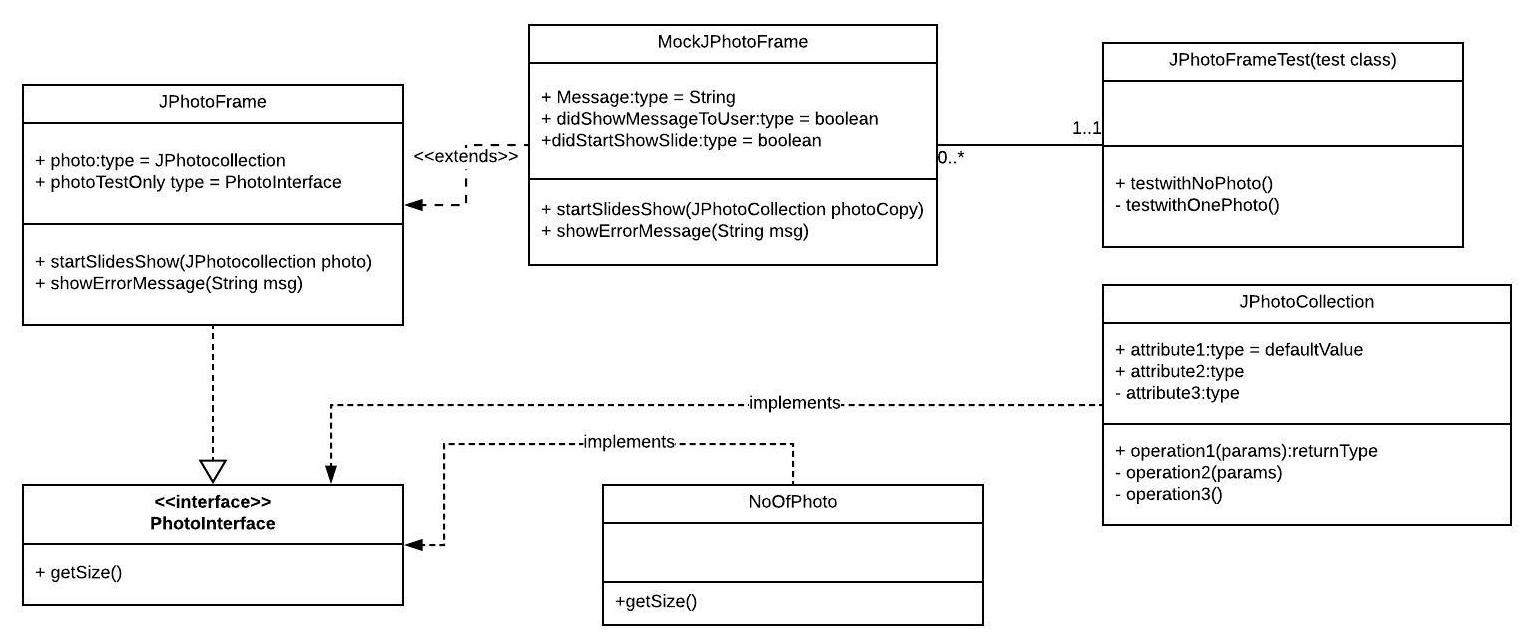
\includegraphics[width=1\linewidth]{uml}
	\caption{UML}
\end{figure}
To perform unit test for "Start Slideshow" button, we extract the related code block from \texttt{actionPerformed()} method in \texttt{JPhotoFrame} class, 
so that some mock objects can call that part of code without executing other parts. Afterwards, in \texttt{JPhotoFrameTest} class we create a subclass \texttt {TestingJPhotoFrame} that extends \texttt{JPhotoFrame} class, 
to instantiate some mock objects. The subclass has some overridden methods which has different utility from its super class, i.e., instead of display slides (if size of photo album > 0) or prompt error message (if size of photo album = 0),
methods in subclass can be overwitten to recording some actual value that help us testing by assserting to some expected value.\\
We perform two test cases to ensure that wo possibilities after clicking is both correct. In the first test case, we have a abstract frame (Not real Photo frame window) which contains no photos and test whether it will show correct error message with expected \texttt{"No photos to show!"}
The second one we have another abstract frame which has exactly one abstract photo in album and test whether it will show the slide (it will not show the slide in real, but returns a \texttt{boolean} value to pretending it is showing). 
More logically, instead of using the \texttt{MockJPhotoFrame} in the test cases we can break dependency by instanciating \texttt{NoOfPhoto}, so that we can get rid of calling other part in \texttt{JPhotoCollection}, 
\begin{figure}[H]
  \centering
  \setlength{\abovecaptionskip}{-0.1in}
  \setlength{\belowcaptionskip}{-0.15in}
	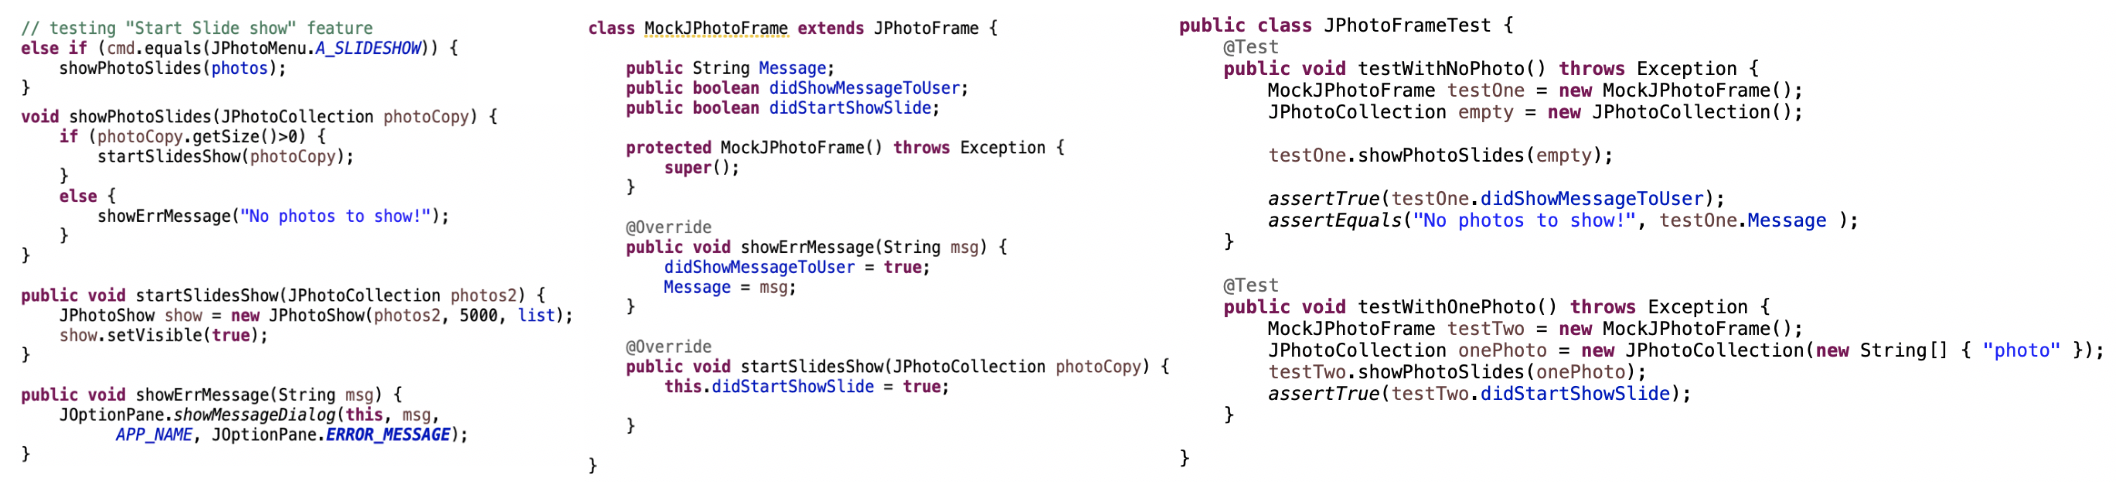
\includegraphics[width=1\linewidth]{codeblock}
	\caption{Extracting behaviour out; Subclass for testing; Unit test class conducting 2 test cases}
\end{figure}
Testing things are all passed in as parameters so that this code is hard to test. In terms of  tradeoffs, instead of using PhotoInterface we instantiate the JPhotoFrame and pass some range string to make the photo size > 0 or we can instantiate the JPhotoFrame by using the default constructor. We make this tradeoff because instantiating the JPhotoFrame does not have a lot of external dependencies and is less time-consuming. By using the interface in a large-scale project,  we might introduce an anonymous bug into the preious code so that it becomes more time-consuming.\\
Testing driven design may change the code structure because a common intuition for the developer is to satisfy the testing rather than implementing good structure. \\[10px]
To add new feature as "Quick Slideshow" we add another button in \texttt{JPhotoMenu} class, as well as another event (\texttt{elseif} block) under \texttt{actionPerformed()} method in \texttt{JPhotoFrame} class, where we perform similar implementation as original Slideshow apart from changing parameters passed into 
\texttt{JPhotoShow} from \texttt{5000} to \texttt{50}, which means reducing time intervals from 5000ms to 50ms. Similar unit tests can be applied and details can be found on GitLab: \\
\href{https://gitlab.doc.ic.ac.uk/jz2618/jphotoalbum.git}{https://gitlab.doc.ic.ac.uk/jz2618/jphotoalbum.git} \\[10px]

\end{document}
